% The last row uses the installed PGF manual's rounding-function examples.
\documentclass[border=2pt]{standalone}
\usepackage{tikz}
\begin{document}
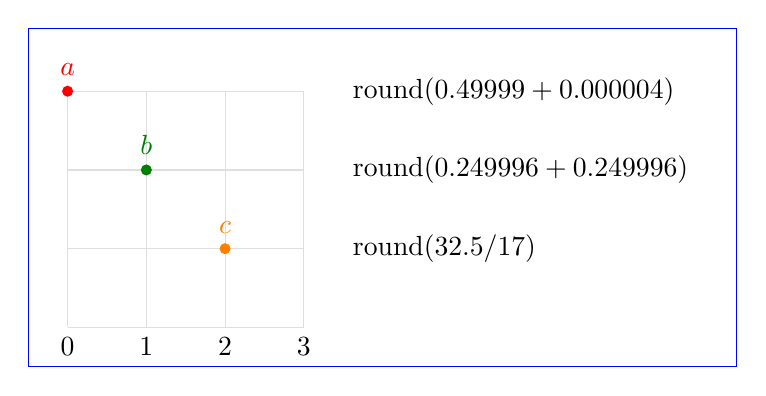
\begin{tikzpicture}
  \draw[blue] (-.5,-.5) rectangle (8.5,3.8);
  \draw[gray!25] (0,0) grid (3,3);
  \foreach \x in {0,1,2,3} \node[below] at (\x,0) {$\x$};
  \node[anchor=west] at (3.5,3) {round$(0.49999+0.000004)$};
  \node[anchor=west] at (3.5,2) {round$(0.249996+0.249996)$};
  \node[anchor=west] at (3.5,1) {round$(32.5/17)$};
  \fill[red] ({round(0.49999+0.000004)},3) circle (2pt) node[above=2pt] {$a$};
  \fill[green!50!black] ({round(0.249996+0.249996)},2) circle (2pt) node[above=2pt] {$b$};
  \fill[orange] ({round(32.5/17)},1) circle (2pt) node[above=2pt] {$c$};
\end{tikzpicture}
\end{document}
